\chapter{Part II(e) - Processor, I/Os, and Exceptions - Example W - 6.2}
\section{Part Ia: Connecitng an Input Peripheral}
Consider a hypothetical processor with the following buses and control signals:
\begin{itemize}
    \item[-] \textbf{A[31:0]}: Address bus
    \item[-] \textbf{D[31:0]}: Data bus
    \item[-] \textbf{AS} (Address Strobe): Active when a valid address is present on \textbf{A[31:0]}.
    \item[-] \textbf{WR} (Write): Active along with \textbf{AS} during a write cycle.
\end{itemize}

The input peripheral consists of 10 buttons numbered from 0 to 9, where:
\begin{itemize}
    \item[] Each button outputs a logic ‘1’ when pressed and ‘0’ otherwise.
    \begin{center}
        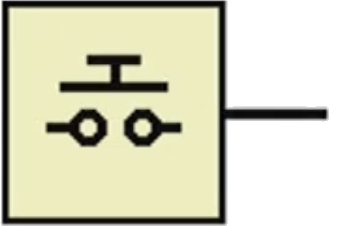
\includegraphics[width=0.10\textwidth]{chapters/chapter2e/images/button.png}
    \end{center}
    \item[] The processor reads the \textbf{state of the buttons} from memory location \texttt{0xFFFF'FFF0}:
    \begin{itemize}
        \item A value of ‘0’ indicates no button is pressed.
        \item A value of ‘1’ indicates at least one button is pressed.
    \end{itemize}
    \item[] The processor reads the \textbf{number of the button pressed} from memory location \texttt{0xFFFF'FFF4}.
\end{itemize}

\section{Bus Protocol}
 \begin{center}
     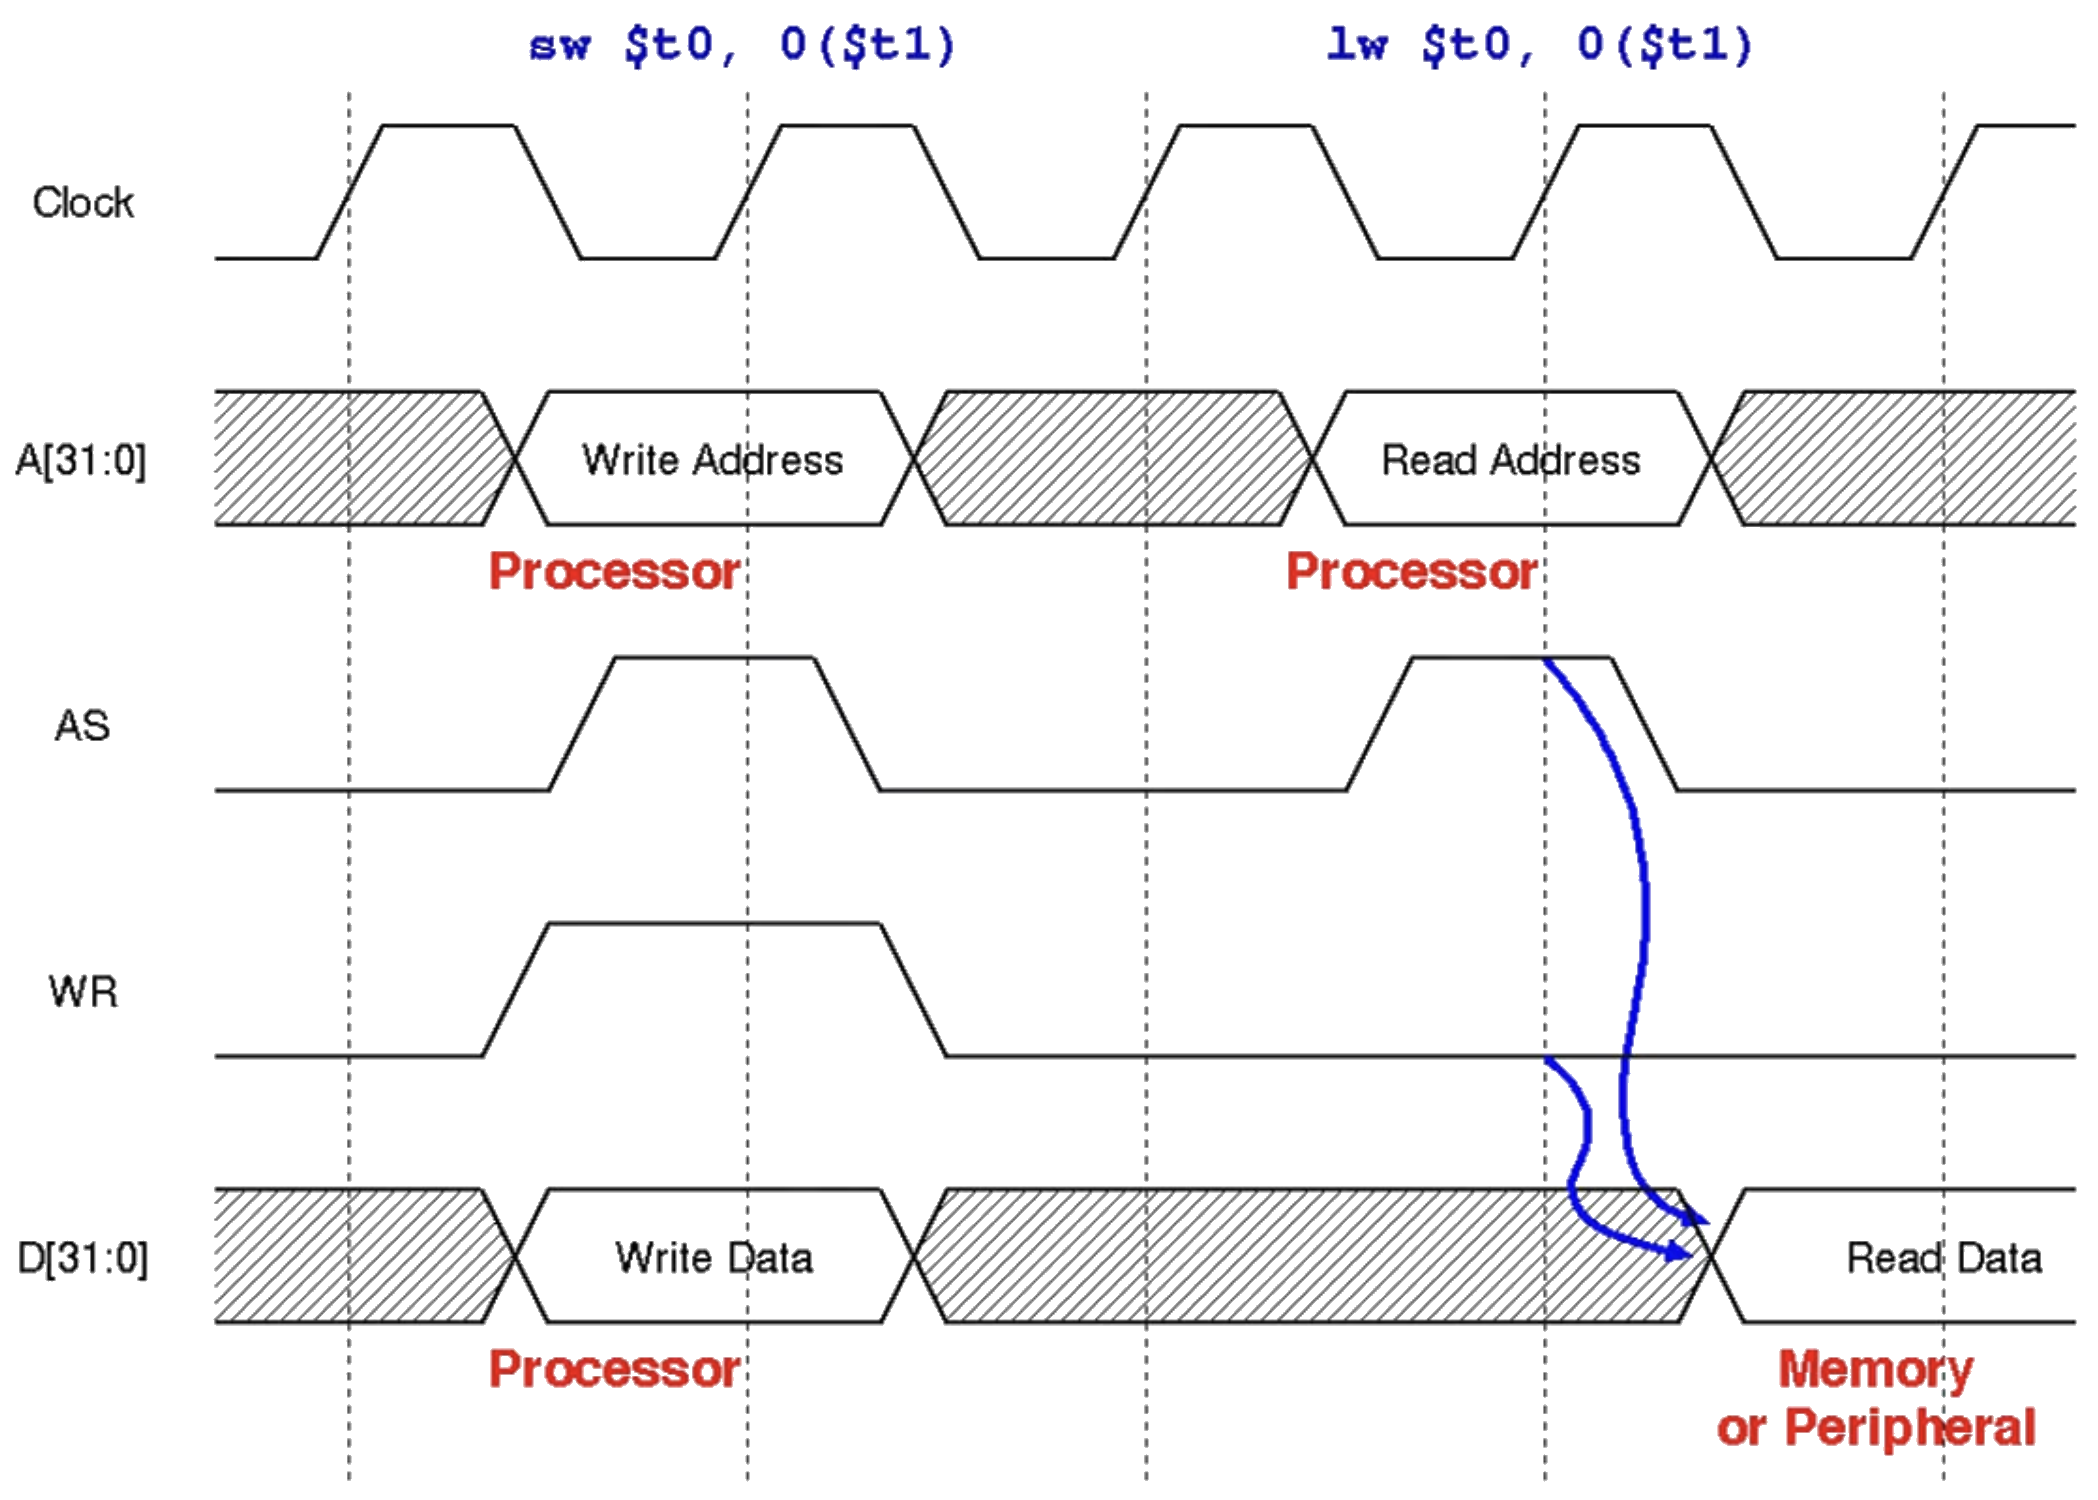
\includegraphics[width=0.45\textwidth]{chapters/chapter2e/images/bus.png}
 \end{center}
\section{Assembling the Circuit}
\textbf{Looking at the timing diagram is really really recommended when assembling a circuit.}
\begin{center}
    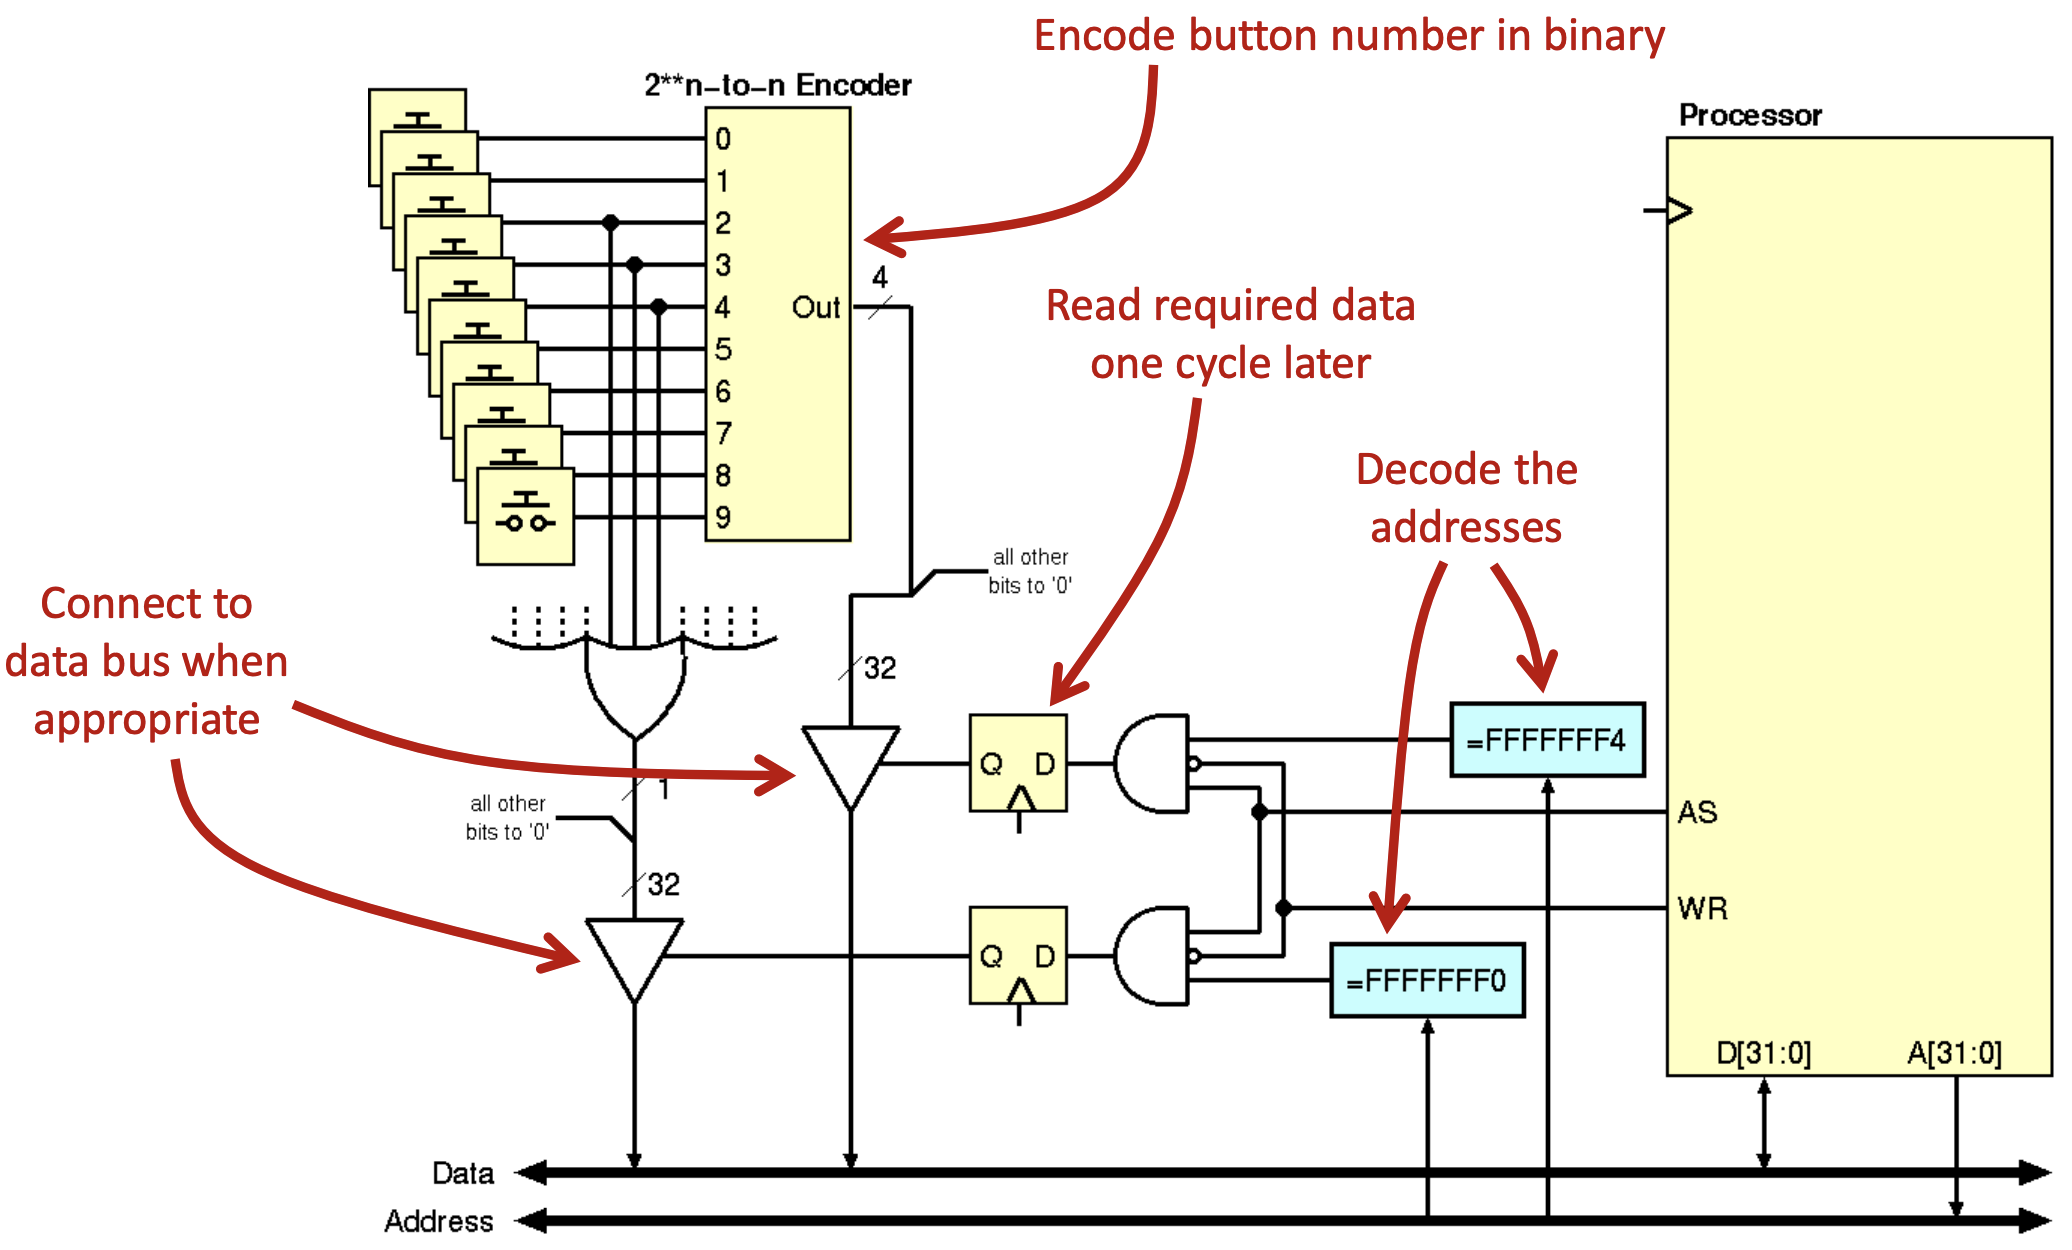
\includegraphics[width=0.65\textwidth]{chapters/chapter2e/images/circuit.png}
\end{center}

The input peripheral circuit connects 10 buttons to the processor, allowing it to detect button presses and identify which button is pressed. Below are the components of the circuit and their purposes:
\begin{itemize}
    \item[-] \textbf{Buttons:} Represent physical inputs numbered 0 to 9. Each button outputs a logic `1` when pressed and `0` otherwise.
    \item[-] \textbf{2\textsuperscript{n}-to-n Encoder:} Converts the 10 individual button signals into a 4-bit output, representing the button number.
    \item[-] \textbf{Address Decoders:} Determine the memory location being accessed (\texttt{0xFFFF'FFF0} or \texttt{0xFFFF'FFF4}) based on the address bus (\textbf{A[31:0]}).
    \item[-] \textbf{Latches (Q):} Store the state of the buttons and the number of the button pressed, enabling stable data retrieval by the processor.
    \item[-] \textbf{Control Signals (\textbf{AS}, \textbf{WR}):} 
    \begin{itemize}
        \item[-] \textbf{AS} (Address Strobe): Ensures the address on \textbf{A[31:0]} is valid.
        \item[-] \textbf{WR} (Write Enable): Activates during write cycles to store data.
    \end{itemize}
    \item[-] \textbf{Data Bus (\textbf{D[31:0]}):} Transfers data between the processor and the peripheral.
\end{itemize}

\section{Part 1b: Reading the Input Ports}
Write a RISC-V program named \texttt{buttons} to poll the state of the input buttons. The program must meet the following requirements:

\begin{itemize}
    \item Every time a button is pressed, the program should call the function \texttt{ShowIt}.
    \item Register \texttt{a0} must contain the ASCII code of the character corresponding to the button pressed. For example:
    \begin{itemize}
        \item Button ``0'' $\rightarrow$ ASCII code 48
        \item Button ``1'' $\rightarrow$ ASCII code 49
        \item Button ``2'' $\rightarrow$ ASCII code 50
    \end{itemize}
    \item The function \texttt{ShowIt} is provided, and you do not need to implement it.
\end{itemize}

\subsection{Software: buttons}
\begin{assembly}
    li s0, 0xFFFFFFF0
poll:    
    lw t0, 0(s0)
    beqz t0, 0(s0)
    lw t0, 4(s0)
    jal showIt
    j poll
\end{assembly}

\section{Part 2a - Connecting an Output Peripheral}
\begin{center}
    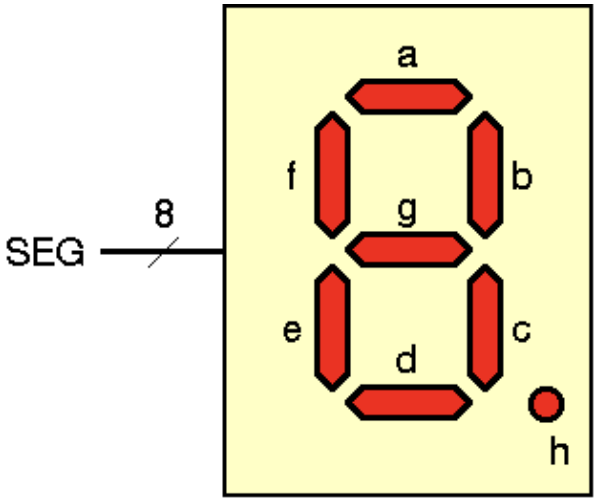
\includegraphics[width=0.15\textwidth]{chapters/chapter2e/images/seg8.png}
\end{center}
\begin{itemize}
    \item[] The peripheral receives an 8-bit signal, \texttt{SEG}, where each bit corresponds to a segment of the display:
    \begin{itemize}
        \item Bit 0 $\rightarrow$ Segment \texttt{a}
        \item Bit 1 $\rightarrow$ Segment \texttt{b}
        \item Bit 2 $\rightarrow$ Segment \texttt{c}, and so on.
    \end{itemize}
    A bit value of \texttt{1} indicates that the corresponding segment is lit.
    \item[] The processor writes a digit to the display by performing a write operation to the memory location \texttt{0xFFFF'FFF8}.
\end{itemize}
\section{Assembling everything}
\begin{center}
    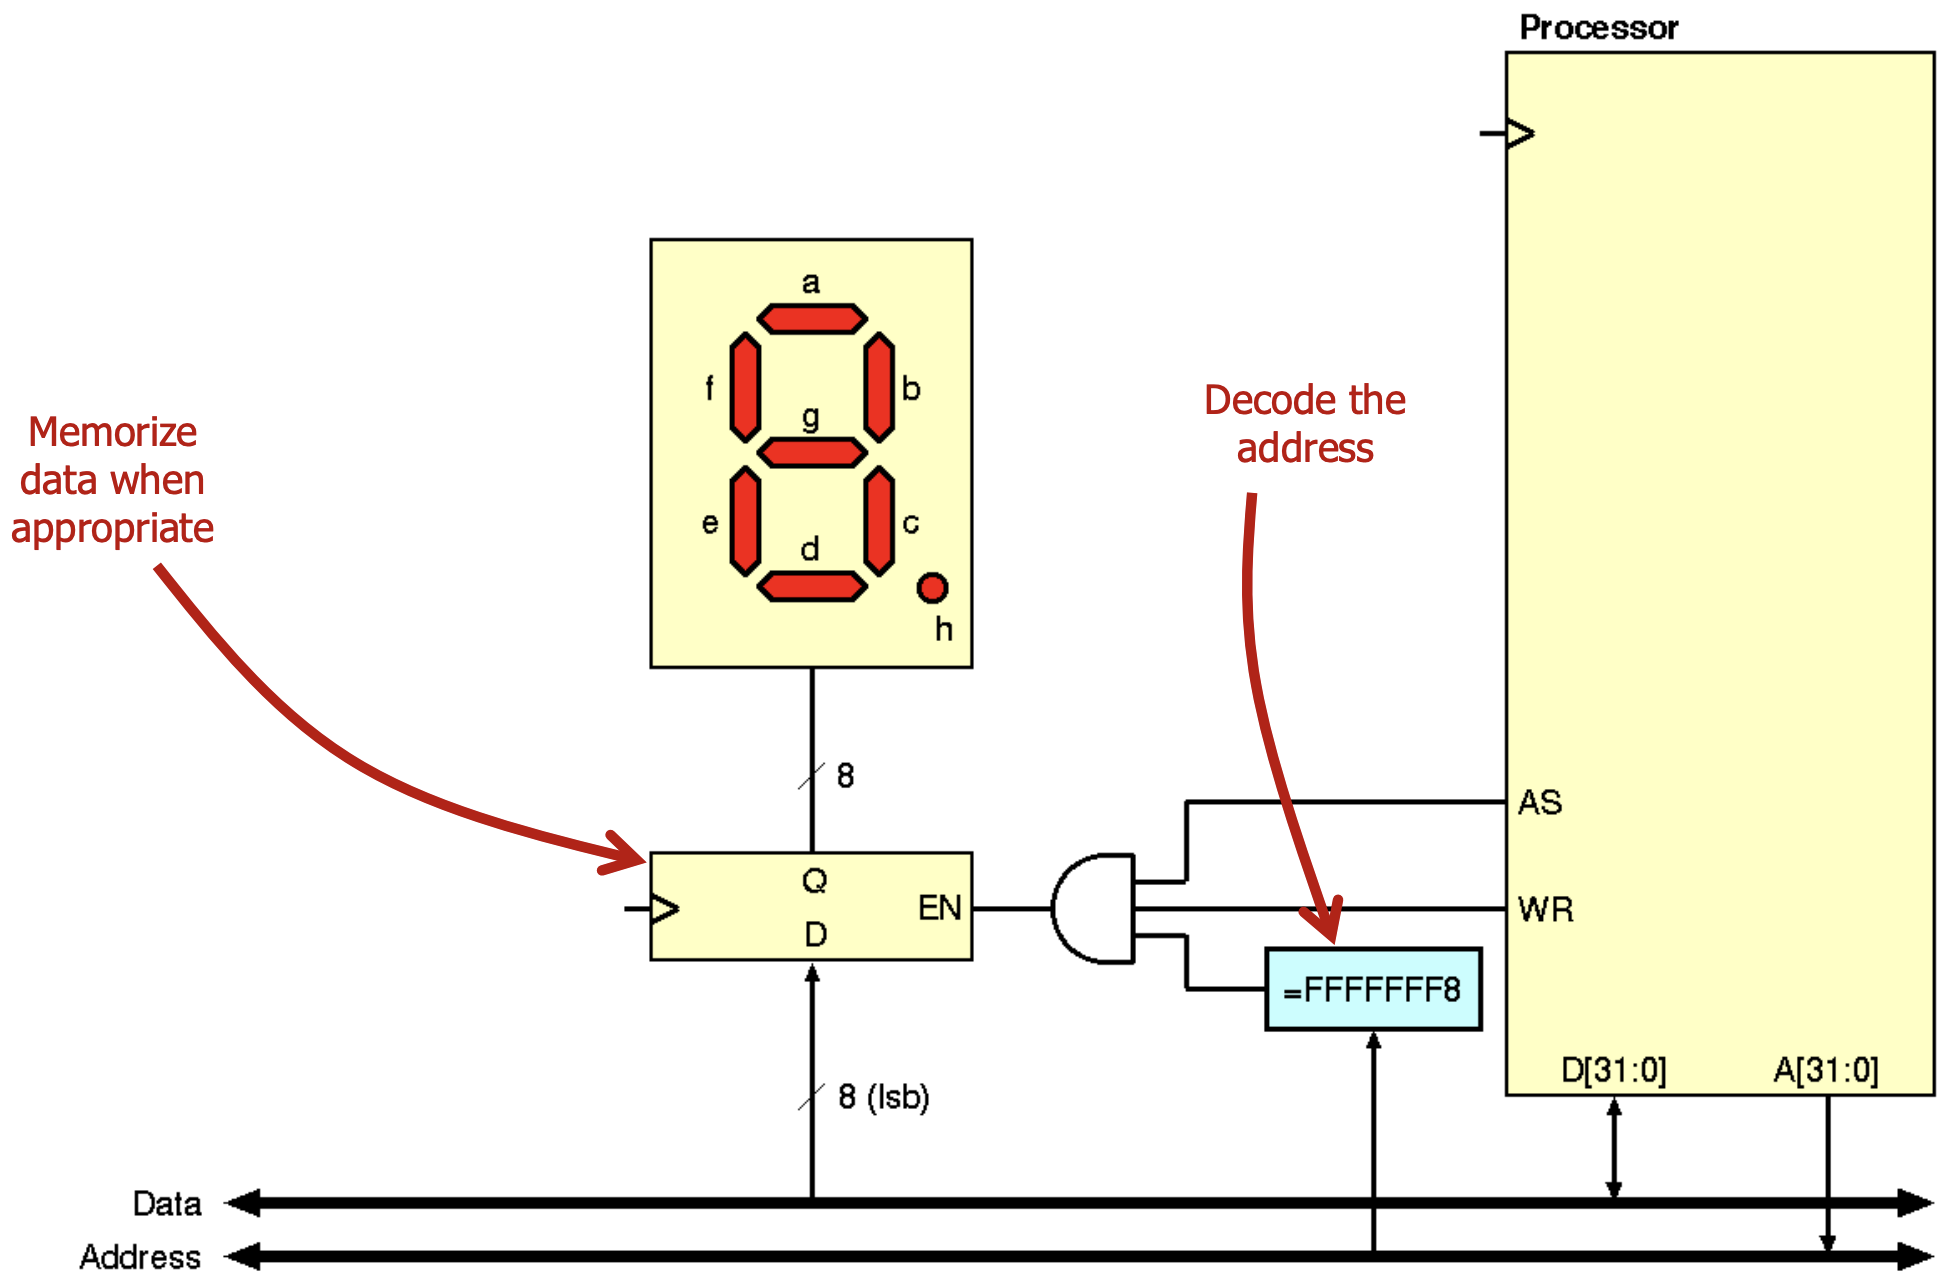
\includegraphics[width=0.65\textwidth]{chapters/chapter2e/images/circuit2.png}
\end{center}

\section{Part 3a: Use Interrupts}
The processor includes three \textbf{Interrupt Priority Level} input pins, denoted as \texttt{IPL[2:0]}, which allow I/O devices to initiate interrupts. The interrupt handling mechanism functions as follows:

\begin{itemize}
    \item[] The binary value on the \texttt{IPL[2:0]} pins determines the \textbf{Priority Level} of the interrupt:
    \begin{itemize}
        \item[-] \texttt{0}: No interrupt request.
        \item[-] \texttt{1}: Lowest priority.
        \item[-] \texttt{7}: Highest priority.
    \end{itemize}
    \item[] An interrupt is \textbf{served only if} its priority level exceeds the current level stored in the processor's special status register.
    \item[] Interrupts at \textbf{Priority Level 7} are always served, as they are non-maskable.
    \item[] Modify the button interface to generate an interrupt with priority level 3 and identifier 0x45 when a button is pressed.
    \item[] The port at memory location 0xFFFF'FFF0 is no longer used.
\end{itemize}

\subsection{Interrupt Acknowledgement Process}

The interrupt acknowledgement process involves a coordinated sequence between the processor and peripheral devices. The key steps are outlined as follows:

\begin{center}
    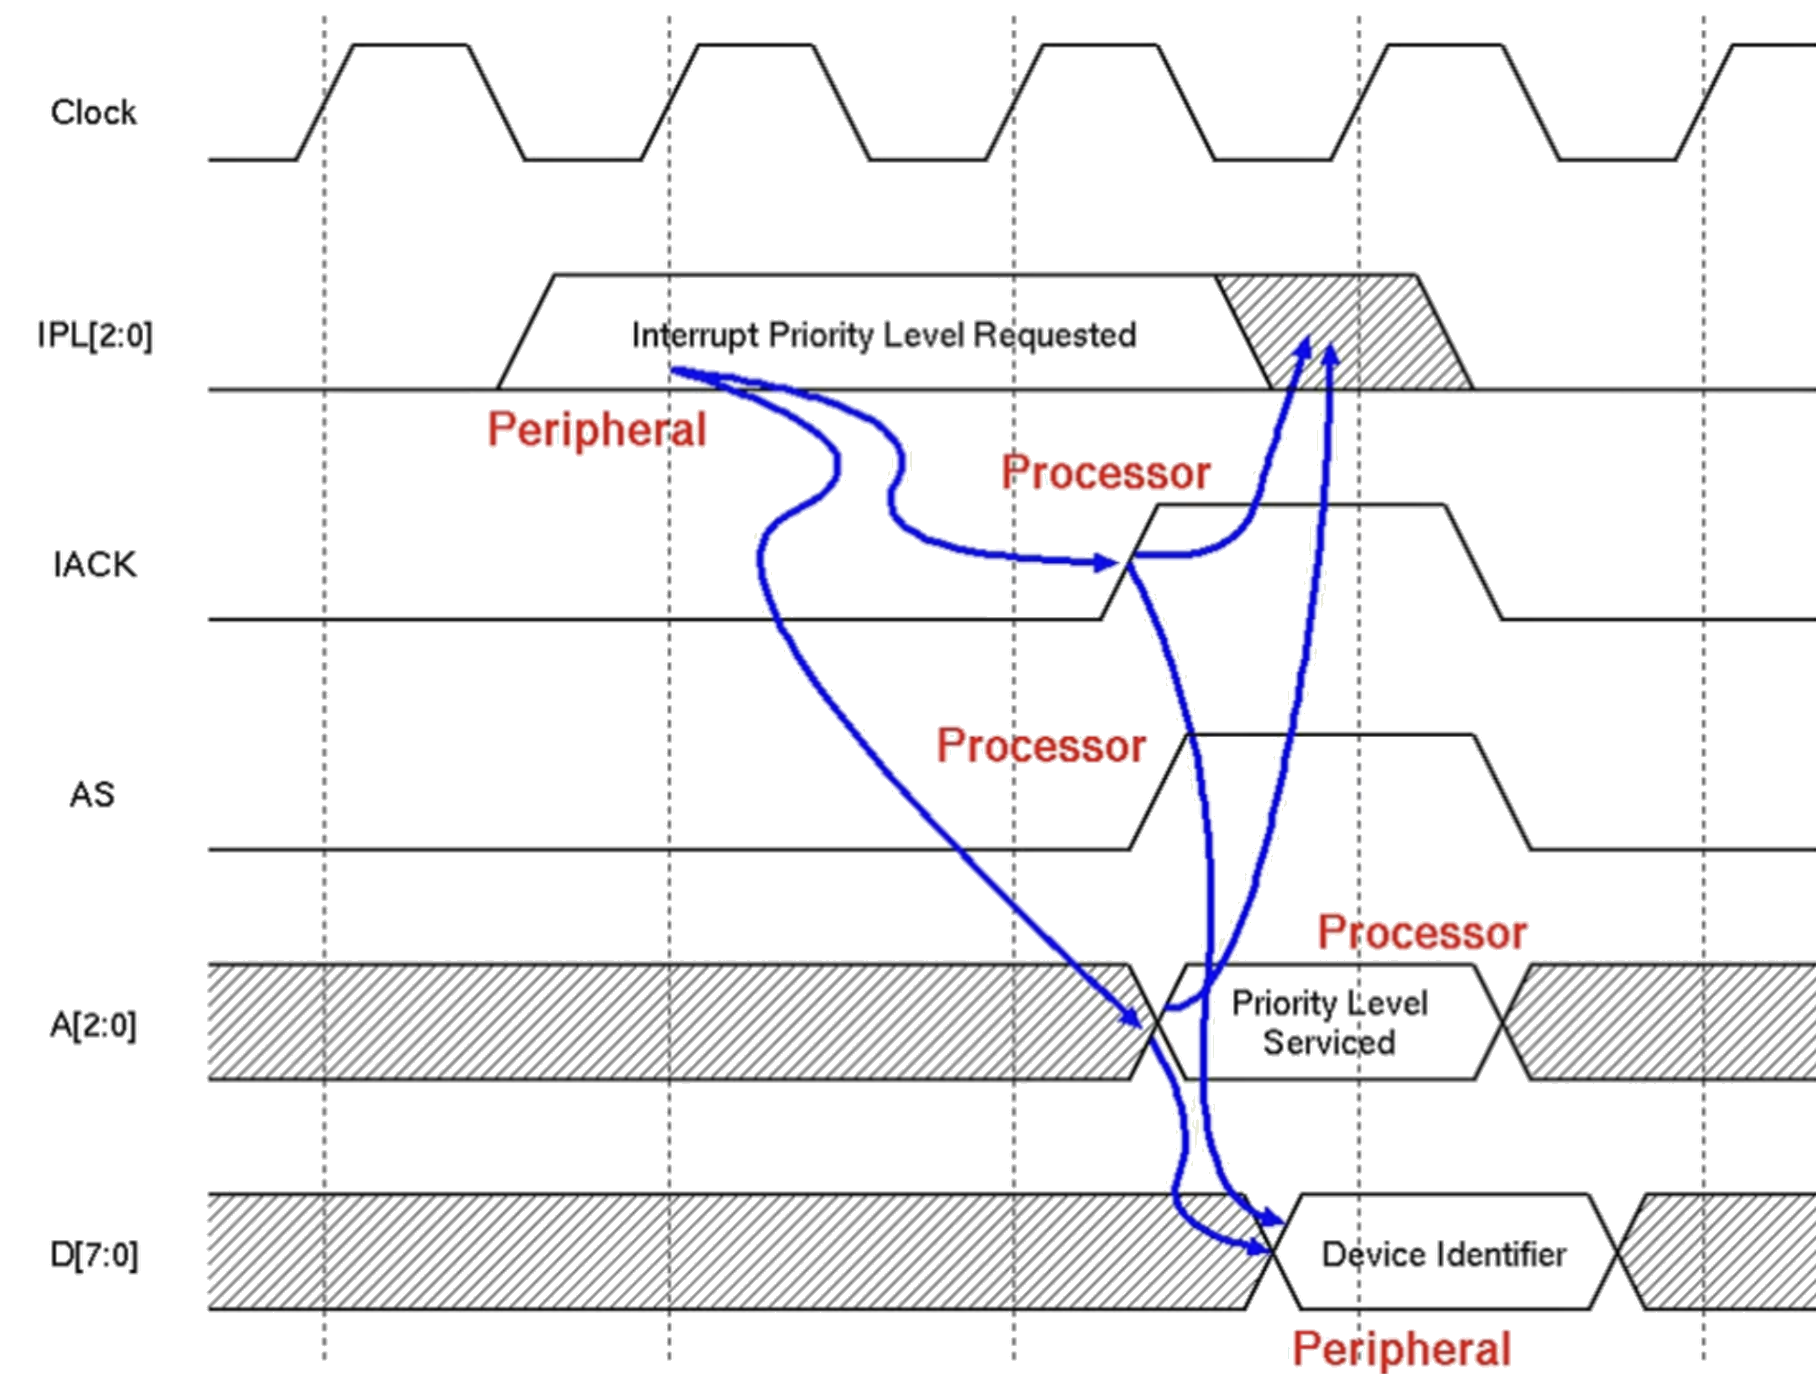
\includegraphics[width=0.45\textwidth]{chapters/chapter2e/images/interrupt_ack.png}
\end{center}
\begin{itemize}
    \item[] The peripheral device asserts an \textbf{Interrupt Priority Level Request} on the \texttt{IPL[2:0]} lines, indicating the interrupt priority level.
    \item[] The processor recognizes the interrupt and initiates an \textbf{Interrupt Acknowledge (IACK)} signal to acknowledge the request.
    \item[] The processor evaluates the priority level of the interrupt:
    \begin{itemize}
        \item[-] If the priority level matches or exceeds the current threshold, the interrupt is serviced.
        \item[-] Otherwise, the interrupt is ignored or deferred.
    \end{itemize}
    \item[] Once the interrupt is acknowledged, the processor asserts the \textbf{Address Strobe (AS)} signal to identify the interrupting device.
    \item[] The peripheral responds by placing the \textbf{Device Identifier} on the \texttt{D[7:0]} data lines for the processor to process.
\end{itemize}
\newpage
\subsection{Solution}
\textit{Final circuit solution with interrupt handling mechanism:} \\
\vspace{10px}
\begin{minipage}[htp]{0.40\textwidth}
    \footnotesize
    \begin{itemize}
        \item \textbf{Retaining the Interrupt Request (IREQ):} 
        The \texttt{IREQ} signal is maintained active until the interrupt is served. This ensures that the request is not lost if the processor is handling a lower-priority task at the time of the interrupt.
    
        \item \textbf{Required Priority Level:} 
        The updated implementation includes a multiplexer that selects the required priority level for the interrupt. This allows the processor to dynamically assess whether the priority of the interrupt request is sufficient to preempt the current task.
    
        \item \textbf{Device Identifier:} 
        The device identifier (\texttt{0x45}) is explicitly encoded and transmitted over the data bus. This provides a clear and efficient way for the processor to identify the source of the interrupt.
    
        \item \textbf{Integration with the Processor:} 
        The processor interacts with the interrupt handling circuitry through the \texttt{IPL[2:0]}, \texttt{IACK}, and \texttt{AS} signals. These signals ensure that the interrupt servicing process aligns with the required priority levels and device identification.
    
        \item \textbf{New Comparator Mechanism:} 
        A comparator checks whether the least significant bits (LSBs) of the address match the expected value (\texttt{=3}). This additional check further validates the interrupt source and enhances system robustness.
    \end{itemize}
\end{minipage}
\hfill
\vline
\hfill
\begin{minipage}[htp]{0.55\textwidth}
    \begin{center}
        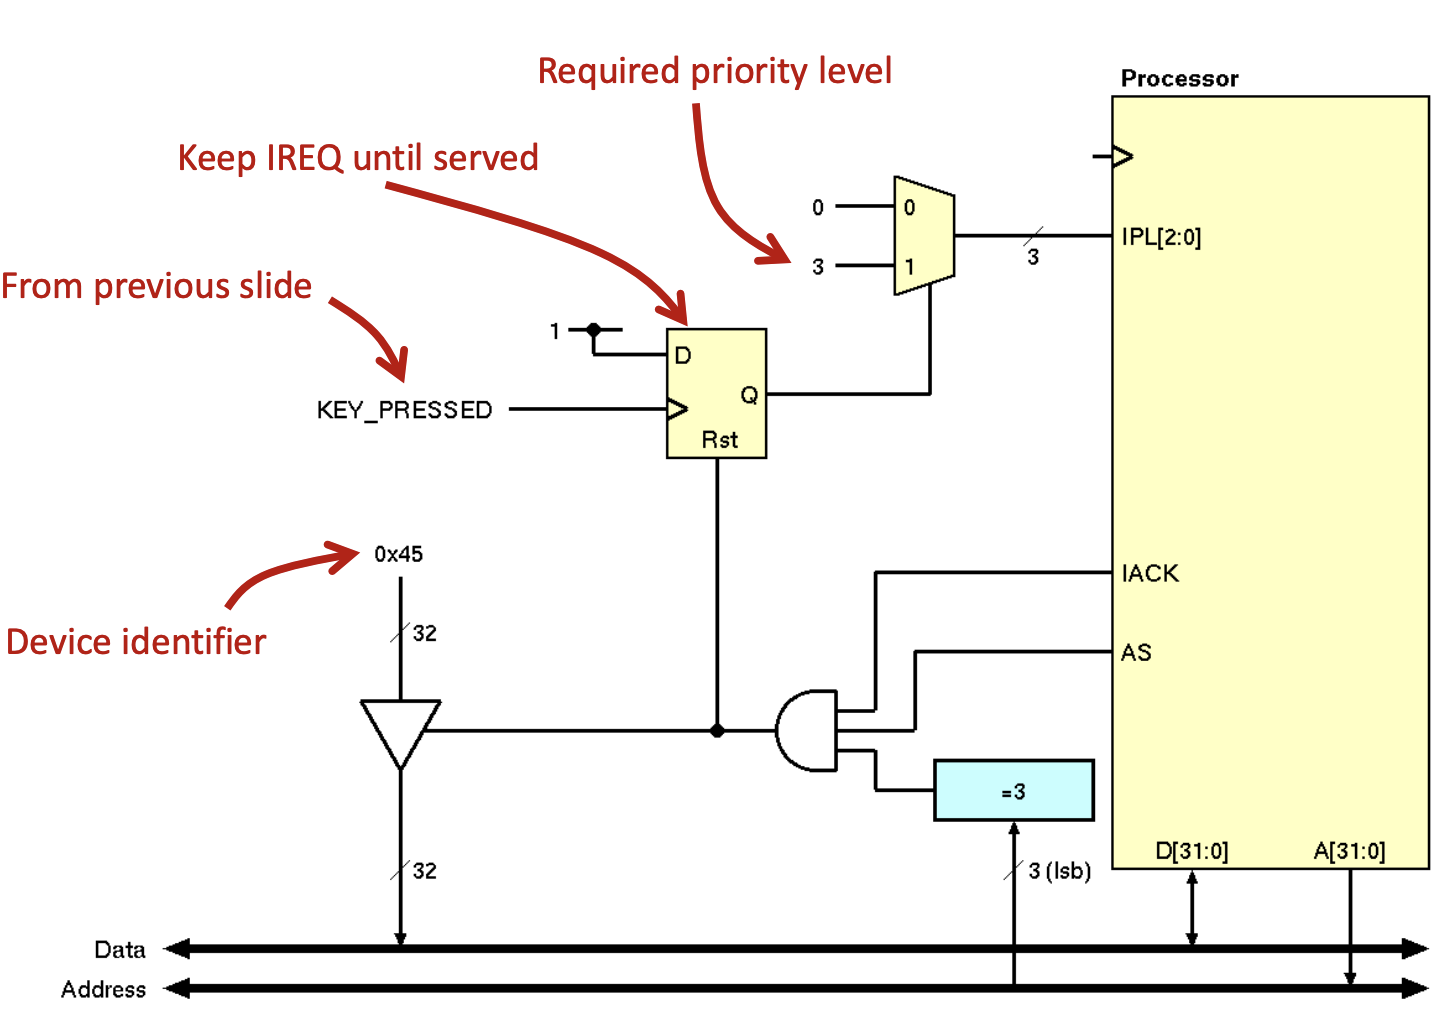
\includegraphics[width=0.85\textwidth]{chapters/chapter2e/images/circuit3.png}
    \end{center}
\end{minipage}

